\subsection{Data schema and models}
Here are the reasoning behind the design of our data schema (See figure \ref{fig:schema}):
\begin{itemize}%[leftmargin=*]
    \item User: it should have username, password and role (user or admin).
    \item Location: it should have name, latitude, longitude and district (i.e. area).
    \item Event: it should have title, reference to location, date (\verb|preDateE|), duration (\verb|progTimeE|), price and presenter.
    \item Favourite: it should have reference to both user and location.
    \item Like: similar to Favourite, it should have reference to both user and event.
    \item Comment: beside reference to user and location, it also need to store the content as a string.
\end{itemize}
\begin{figure}[h]
    \centering
    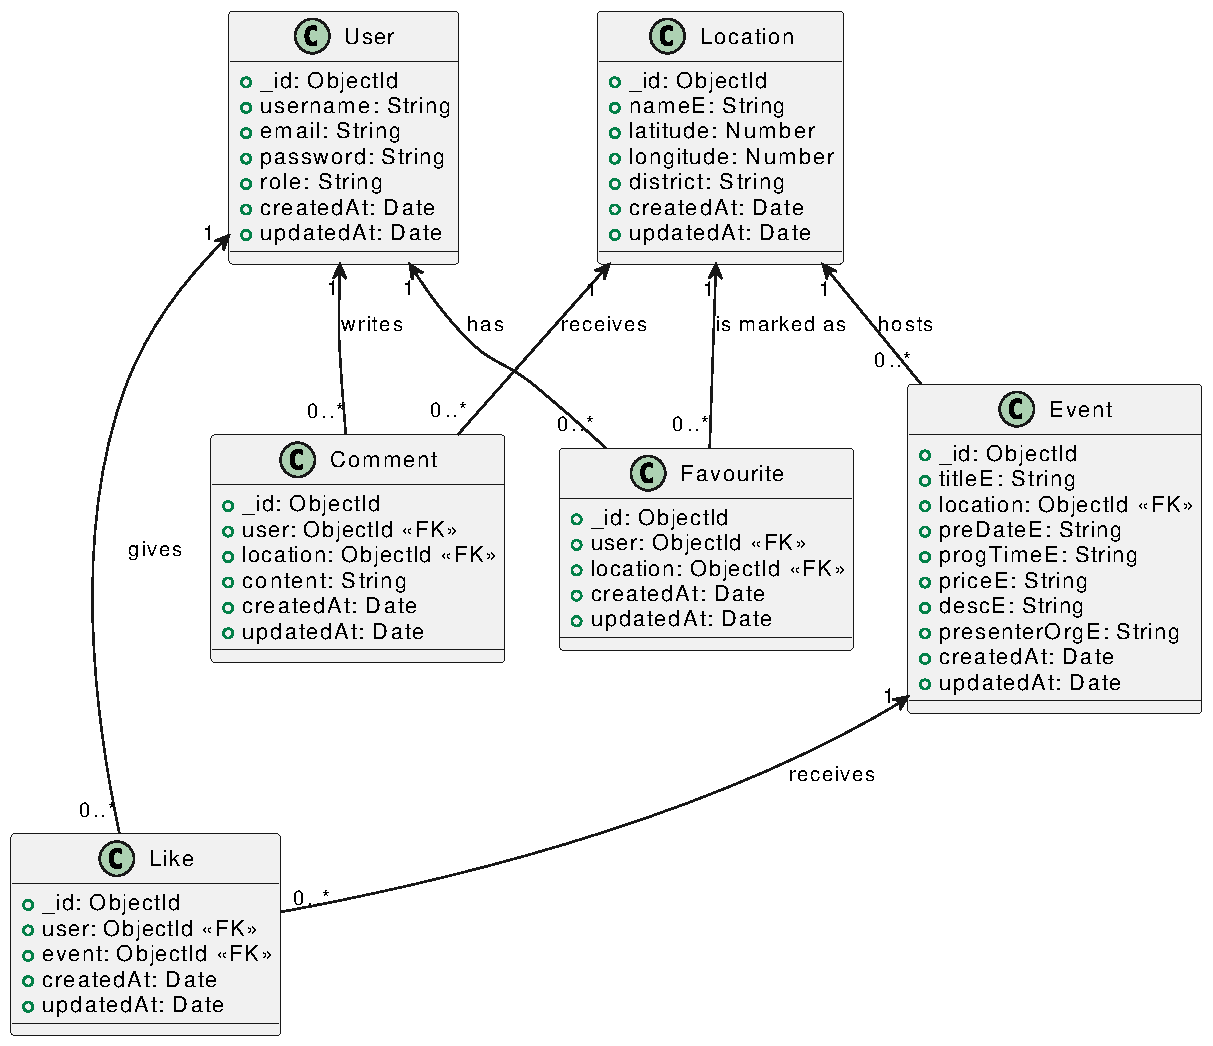
\includegraphics[width=0.8\textwidth]{figures/schema/schema.pdf}
    \caption{UML Class diagram for the data schema}
    \label{fig:schema}
\end{figure}